\documentclass[letterpaper, reqno,11pt]{article}
\usepackage[margin=1.0in]{geometry}
\usepackage{color,latexsym,amsmath,amssymb,graphicx, float}
\usepackage{hyperref}

\hypersetup{
colorlinks=true,
linkcolor=magenta,
filecolor=magenta,
urlcolor=cyan,
}

\graphicspath{ {images/} }

\begin{document}
\pagenumbering{arabic}
\title{PHYS 304 Assignment 4}
\date{08/02/22}
\author{Xander Naumenko}
\maketitle

{\noindent\bf Question 1a.} 
\[
\int_{-\infty}^{\infty}\Phi^*\Phi dx=A^2\int_{-\infty}^{\infty}\left( 9|\phi_0|+16|\phi_1|+12\phi_0^*\phi_1+12\phi_0\phi_1^* \right) dx=25\implies A=\frac{1}{5}
.\]

{\noindent\bf Question 1b.} Since the given intial conditions is just the superposition of eigenstates, it will continue to be. Then we have that: 
\[
\Psi(x, t)=\frac{1}{5}(3\psi_0(x)e^{-i(\frac{1}{2}\omega t)}+4\psi_1(x)e^{-i(\frac{3}{2})\omega t})
\]
\[
=\frac{1}{5}\left( \frac{m\omega}{\pi \hbar} \right)^{1 /4}(3e^{-\xi^2 /2}e^{-i(\frac{1}{2}\omega t)}+4\frac{1}{\sqrt{2} }2\xi e^{-\xi^2 /2}e^{-i(\frac{3}{2})\omega t}), \xi=\sqrt{\frac{m\omega}{\hbar}} x
.\]
Next calculate the absolute value: 
\[
|\Psi(x, t)|^2=\frac{1}{5}\left( 9(\psi_0(x))^2+16(\psi_1(x))^2+12\psi_1\psi_0 e^{-i\omega t}+12\psi_1\psi_0 e^{i\omega t} \right) 
\]
\[
=\frac{1}{25}\left( 9(\psi_0(x))^2+16(\psi_1(x))^2+24\psi_0\psi_1\cos(\omega t) \right)
.\]

{\noindent\bf Question 1c.} 
\[
\left<x \right>=\int_{-\infty}^{\infty}\Psi^{*}(x, t)x\Psi(x, t)dx=\frac{9}{25}\left<\psi_0 \right>+\frac{16}{25}\left<\psi_1 \right>+\int_{-\infty}^{\infty}\frac{24}{25}x\psi_1\psi_2\cos(\omega t)dx
\]
\[
=0+0+\frac{24}{25}\cos(\omega t)\sqrt{\frac{\hbar}{m\omega\pi}} \int_{-\infty}^{\infty}\frac{2}{\sqrt{2} }\xi^2 e^{-\xi^2}d\xi=\frac{24}{25}\cos(\omega t)\sqrt{\frac{\hbar}{m\omega}}\sqrt{\frac{2}{\pi}} \int_{-\infty}^{\infty}\xi^2 e^{-\xi^2}d\xi
\]
\[
=\frac{24}{25}\cos(\omega t)\sqrt{\frac{\hbar}{m\omega}}\sqrt{\frac{2}{\pi}}\sqrt{\frac{\pi}{4}} =\sqrt{\frac{\hbar}{2m\omega}}\frac{24}{25}\cos(\omega t)
.\]
\[
\left<p \right>=m\frac{d\left<x \right>}{dt}=-\frac{24}{25}\sqrt{\frac{\hbar m\omega}{2}}\sin(\omega t)
.\]
Verifying Ehrenfest's theorem: 
\[
\frac{d\left<p \right>}{dt}=\frac{24}{25}\sqrt{\frac{\hbar m\omega}{2}}\cos(\omega t)=m\omega \left<x \right>=\left<-\frac{dV}{dx} \right>
\]
as expected. 

{\noindent\bf Question 1d.} The probabilities are the square of the coefficients, associated with that eigenstate. Thus the probability of having energy $ E_0=\frac{1}{2}\hbar\omega$ is 
\[
    (\frac{3}{5})^2=\frac{9}{25}
.\]
The probability of having energy $ E_1=\frac{3}{2}\hbar\omega$ is 
\[
    (\frac{4}{5})^2=\frac{16}{25}
.\]

{\noindent\bf Question 2.} The probability is the integral of the square of the wavefunction, and because the wavefunction is symmetric about $0$ we have: 
\[
P=2\int_{\sqrt{\frac{\hbar}{m\omega}}}^\infty \left( \frac{m\omega}{\pi\hbar} \right)^{1 /2}e^{-\frac{m\omega x}{\hbar}}dx
\]
\[
=2\left( \frac{m\omega}{\pi\hbar} \right)^{\frac{1}{2}}\left( \frac{\hbar}{m\omega} \right)^{\frac{1}{2}}  \int_{1}^{\infty}e^{-\xi^2}d\xi
.\]
Solving this numerically with WolframAlpha we get that this integral is equal to $P=0.157$. 

{\noindent\bf Question 3a.} 
\[
\int_{-\infty}^{\infty}A^2e^{-2ax^2}dx=A^2 \sqrt{\frac{\pi}{2a}}=1\implies A=\left( \frac{2a}{\pi} \right)^{1 /4}
.\]

{\noindent\bf Question 3b.} From the textbook the general expression for the wavefunction of a free particle is 
\[
\frac{1}{\sqrt{2\pi} }\int_{-\infty}^{\infty}\phi(k)e^{ikx}dk, \phi(k)=\frac{1}{\sqrt{2\pi} }\int_{-\infty}^{\infty}\Psi(x, 0)e^{-ikx}dx
\]
\[
\phi(k)=\frac{1}{\sqrt{2\pi} }\int_{-\infty}^{\infty}e^{-ax^2-ikx}dx
.\]
Let $y=\sqrt{a} (x+\frac{b}{2a})=\sqrt{a} (x+\frac{ik}{2a})$. Then the integral becomes 
\[
\phi(k)=A\frac{1}{\sqrt{2\pi} }\int_{-\infty}^{\infty}e^{-y^2+\frac{k}{4a}}dy=\frac{e^{-k^2 /4a}}{\sqrt{2a} }\left( \frac{2a}{\pi} \right)^{1 /4}=\frac{e^{-k^2 /4a}}{(2a\pi)^{1 /4} }
.\]
Then the expression for the wavefunction is 
\[
\Psi(x, t)=\frac{1}{\sqrt{ 2\pi}(2a\pi)^{1 /4} }\int_{-\infty}^{\infty}e^{-\left(k^2 \left(1/4a+\frac{i\hbar}{2m}t\right)-ixk\right)}dk
.\]
Let $j=\frac{1}{\sqrt{1/4a+\frac{i\hbar}{2m}t}}\left( k+\frac{1/4a+\frac{i\hbar}{2m}t}{2ix} \right)\implies k^2\left( 1/4a+\frac{i\hbar}{2m}t \right) -ikx=j^2+\left( \frac{x^2}{1 /a+\frac{2i\hbar}{m}t} \right) $. Plugging this back into the integral: 
\[
\Psi(x, t)=\frac{1}{\sqrt{ 2\pi}(2a\pi)^{1 /4} }\frac{1}{\sqrt{1/4a+\frac{i\hbar}{2m}t}}\int_{-\infty}^{\infty}e^{-j^2-\left( \frac{x^2}{1 /a+\frac{2i\hbar}{m}t} \right)}dj
.\]
Let $\gamma=\sqrt{1+(2i\hbar at /m)} $. Then the above integral reduces to (taking the normal distribution integral known to be $ \sqrt{\pi} $): 
\[
\Psi(x, t)=\frac{1}{\sqrt{ 2}(2a\pi)^{1 /4} }\frac{2\sqrt{a}}{\gamma}e^{-ax^2 /\gamma^2}
\]
\[
\Psi(x, t)=\left(\frac{2a}{\pi}\right)^{1 /4}\frac{1}{\gamma}e^{-ax^2 /\gamma^2}
.\]

{\noindent\bf Question c.} Multiplying the above expression with its conjugate: 
\[
|\Psi(x, t)|^2=\sqrt{\frac{2a}{\pi}}\frac{1}{\sqrt{(1+(2i\hbar at /m)(1-(2i\hbar at /m)} }e^{-ax^2 /(1+(2i\hbar at /m))}e^{-ax^2 /(1-(2i\hbar at /m)) }
\]
\[
=\sqrt{\frac{2}{\pi}}we^{-2w^2x^2} 
.\]
As can be seen in figure \ref{fig:q3ci} and \ref{fig:q3cii}, the wavepacket spreads out over time. Note that the values used in the graphs are arbitrary and are just meant to show the trend over time. 

\begin{figure}[htpb]
    \centering
    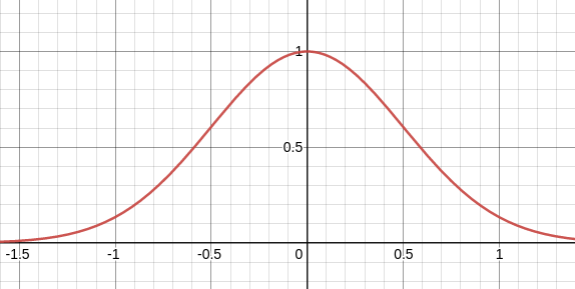
\includegraphics[width=0.8\textwidth]{q3ci.png}
    \caption{Question 3 graph at $t=0$. }
    \label{fig:q3ci}
\end{figure}

\begin{figure}[htpb]
    \centering
    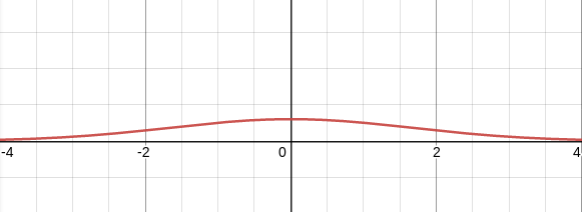
\includegraphics[width=0.8\textwidth]{q3cii.png}
    \caption{Question 3 graph at $t\to\infty$. }
    \label{fig:q3cii}
\end{figure}

{\noindent\bf Question 3d.} The expressian is a Gaussian centered at $x=0$, so $\left<x \right>=0$.
\[
\left<x^2 \right>=\int_{-\infty}^{\infty}\sqrt{\frac{2}{\pi}}wx^2 e^{-2w^2x^2}dx=\sqrt{\frac{2}{\pi}} \sqrt{\frac{\pi}{2w^2}} \frac{w}{4w^2}=\frac{1}{4w^2}
.\]
\[
\left<p \right>=m\frac{d\left<x \right>}{dt}=0
.\]
\[
\left<p^2 \right>=\int_{-\infty}^{\infty}\frac{2}{\pi}\left( w e^{-2w^2x^2} \right)^* \frac{d^2}{dx^2}\left( we^{-2w^2x^2} \right)  dx=h^2a
.\]
\[
\sigma_x=\frac{1}{2w}
.\]
\[
\sigma_p=h\sqrt{h\sqrt{a} } 
.\]

{\noindent\bf Question 3e.} The uncertainty principle does hold, and in fact is exactly equal to the limit when $t=0$: 
\[
\sigma_x\sigma_p=\frac{h\sqrt{a} }{2w}=\sqrt{1+(2\hbar ta /m)^2} \frac{\hbar}{2}\geq \hbar /2
.\]

{\noindent\bf Question 4.} The given potential gives the boundary condition that $\psi(0)=0$. Thus the allowed energies are those corresponding to odd wavefunctions, i.e. $E=(2(n-1)+\frac{1}{2})\hbar\omega, n\in\mathbb{N}$. 





\end{document}
